\chapter{Planteamiento de la Solución}
\label{cap:planteamiento}
\section{Planteamiento inicial}

Una vez vistas las diferencias esenciales entre el sistema original que hemos heredado y las ampliaciones que hemos realizado durante el desarrollo del presente trabajo, se tratará las ideas iniciales de cómo pensábamos realizar el trabajo, indicando desde el punto de vista técnico, organizativo y general, la manera de afrontar este proyecto.

En cuanto a la organización, la planificación inicial era clara: invertir la mayor parte de los primeros meses investigando el proyecto, y a partir del final del primer cuatrimestre y durante todo el segundo cuatrimestre, realizar el trabajo de desarrollo completo del proyecto.

El tema de este TFG fue propuesto por los alumnos, sin una idea clara sobre qué objetivos podría tener el presente trabajo, pero sabiendo que el tema de las simulaciones multiagente es un campo muy interesante en el que profundizar. Durante estos primeros meses se realizaron lluvias de ideas y propuestas para los objetivos. Algunos de los primeros objetivos consistían en añadir funcionalidades a la aplicación o permitir a los usuarios modificarla más, pero decidimos cambiar de objetivos para poder hacer la aplicación ya existente, más fácil de usar para perfiles no técnicos, así como centrarnos en extender ciertas funcionalidades para que sean más útiles para este tipo de perfiles, en lugar para programadores.

Entre las complejidades que se encontraron durante esta primera fase de investigación, se destacan las inconsistencias entre versiones de ciertas tecnologías, la comprensión de todo el código existente, o el aprendizaje de las tecnologías usadas en el desarrollo del proyecto, entre otras muchas. Además, al investigar sobre el tema, esta fue la fase en la que se desarrolló el capítulo del Estado de la Cuestión, lo que ayudó a tomar otra perspectiva acerca del proyecto.

Durante la segunda fase, una vez definidos y validados los primeros objetivos, e comenzó con todo el desarrollo del sistema. Caba destacar que en esta sección, muchas reconsideraciones tuvieron que ser realizadas, además de multitud de cambios en el código original como adaptaciones para que funcionen los nuevos cambios. Todo esto está explicado en las siguientes secciones.

En el transcurso de ambas fases, tuvimos reuniones regularmente con nuestros tutores, supervisando el estado del sistema, así como los avances, problemas y consideraciones que tuviéramos que tener en cuenta. En un principio estas reuniones eran más espaciadas en el tiempo, haciendo una o dos al mes, y en la fase de desarrollo, donde avanzábamos más rápido, las reuniones eran semanales o cada dos semanas para estar al día del proyecto.



\subsection{Estado tecnológico inicial del sistema}

En esta sección se analizará, a grandes rasgos, el estado inicial desde el punto de vista técnico del proyecto. Es decir, el diseño y situación que había inicialmente para ejecutar el sistema, para que en las próximas secciones se entiendan los cambios realizados y el porqué de estos.

En cuanto al diseño, originalmente, existían 2 backends. El primero de ellos era el backend de Django, el cual era el encargado de gestionar todas las llamadas del frontend, o interfaz, que inicialmente no eran muchas, ya que el frontend solamente servía como apoyo para poder visualizar las simulaciones. 

El segundo backend era el de reverie, como lo llaman los autores del código. Este se encargaba de procesar todos los comandos que los usuarios deseaban ejecutar, calculaba el resultado de estos y se comunicaba con el backend de django para que procesase el resultado de las ejecuciones y se reflejara en la interfaz.

\begin{figure}[h]
	\centering
	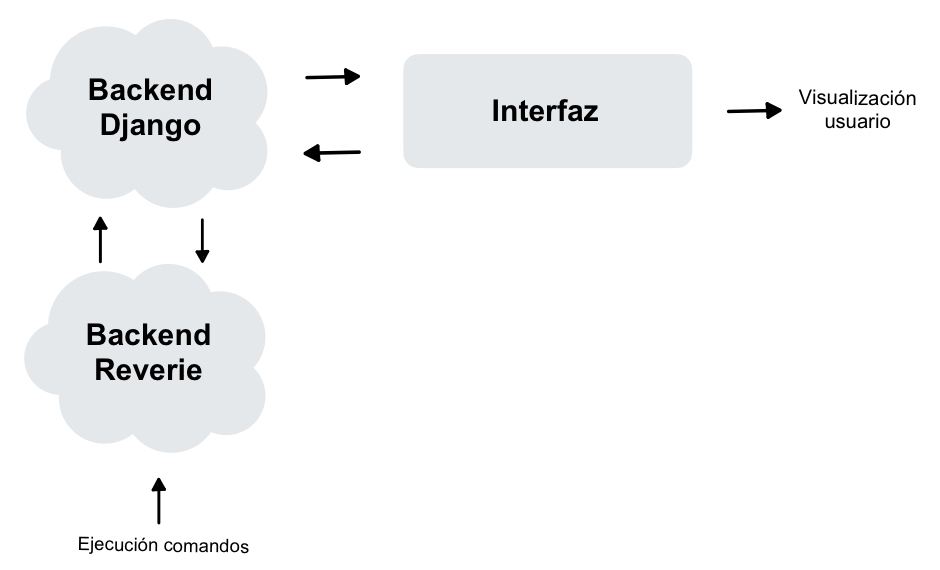
\includegraphics[width = 0.9\textwidth]{Imagenes/Vectorial/disenoSistemaOriginal.jpeg}
	\caption{Diseño del sistema original}
	\label{fig:sistemaOriginal}
\end{figure}

Como se puede ver en la figura \ref{fig:sistemaOriginal}, se ve reflejado el estado del sistema desde el punto del diseño. El flujo habitual sería el siguiente:

\begin{enumerate}
	\item El usuario iría a la terminal en la que se está ejecutando el backend de reverie (que gestiona todas las llamadas a los modelos de lenguaje) y ejecutaría alguno de los comandos (run, whisper, exit, save...)
	
	\item El backend de reverie realizaría la serie de llamadas al modelo de lenguaje pertinentes, así como la organización de las respuestas y almacenamiento de las mismas, y pasaría el resultado de la ejecución al backend de django
	
	\item El backend de Django, con la nueva información obtenida de reverie, adaptaría la información a un formato para que pueda ser procesado en el frontend
	
	\item Se procesaría la información de django en el frontend y se enseñaría al usuario final. Como se ha mencionado, el usuario no podría interactuar con esta información para realizar llamadas al backend desde la interfaz, sino que tendría que acudir a la terminal de reverie para comunicarse
	
\end{enumerate}

También es importante resaltar que para realizar acciones como crear una simulación, ver una simulación existente o interactuar con ella, todas las acciones debían ser realizadas mediante la terminal. La interfaz estaba relegada únicamente a mostrar el resultado de la simulación.

\section{Ajustes y reconsideraciones}

En esta sección se tratarán las adaptaciones que se han ido adoptando durante el desarrollo del proyecto, indicando así cómo han ido cambiando distintas facetas del sistema, tanto en su planificación como en su implementación técnica.

Este análisis permitirá comprender mejor la evolución del proyecto, los desafíos enfrentados y las soluciones implementadas. Además, revelará la capacidad de adaptación y el aprendizaje continuo que han sido fundamentales para el éxito del proyecto.

\subsection{Cambios en los objetivos}

Inicialmente, se fijaron una serie de objetivos sin tener un conocimiento claro sobre la arquiterctura y funcionamiento del sistema. Estos objetivos estaban enfocados en la extensibilidad y modificación de lo previamente existente. A grandes rasgos, los objetivos inicialmente marcados eran los siguientes:

\begin{enumerate}
	\item Añadir uno o varios mapas complementarios a mayores del existente, además de poder modificar las apariencias, nombres y personalidades de los agentes de la simulación
	
	\item Permitir la interacción directa con los agentes y el entorno, pudiendo clicar directamente sobre el mapa y que se reconociese el objeto que se estaba indicando, para así poder modificar su estado (indicar que se está quemando el objeto, por ejemplo)
	
	\item Permitir a los usuarios utilizar su propio modelo del lenguaje, ya sea descargado en local o empleando diferentes APIs externas alternativas al modelo del lenguaje original
\end{enumerate}

Tras evaluar todo el sistema, se decidió pivotar sobre estos objetivos iniciales, ya que conllevaban una gran cantidad de trabajo y apenas aportaban valor añadido al programa original, por lo que se propusieron unos nuevos objetivos, sobre los cuales se ha construído la base de los objetivos finales que se pueden consultar en la introducción de este documento. El resultado de pivotar los objetivos fue, en líneas generales, el siguiente:

\begin{enumerate}
	\item Modificación de las personalidades de los personajes, enfocándose así en la importancia de crear nuevas simulaciones con distintas relaciones sociales, siendo agnósticos al mapa e imagen de los agentes, ya que cambiar esto no aporta tanto valor
	
	\item Interacción en tiempo real con los agentes, mediante un menú en el que poder entrevistar al personaje, así como crearle inquietudes y nuevas memorias para ver cómo reacciona
	
	\item Generación automática de resúmenes
	
	\item Englobar todas las funcionalidades en una interfaz sencilla e intuitiva
\end{enumerate}

\subsection{Limpieza de archivos del repositorio}
\label{limpiezaArchivos}

Al haber heredado el sistema original, realizado por terceros, pudimos apreciar que este, además de no ser extensible, tenía multitud de carpetas, archivos y funciones que no estaban siendo utilizados a día de hoy para nada en el proyecto, o que habían sido utilizados únicamente para depurar el código y lo habían olvidado. Por ello, decidimos limpiar todos estos datos innecesarios y dejar el sistema más limpio y sencillo, para que sea más sencilla la extensibilidad del mismo en el futuro.

En esta sección hemos recogido algunas de estas piezas de código que hemos eliminado, explicando qué hacían y el porqué de su eliminación:

\begin{itemize}
	\item \textbf{Carpeta \textit{path\_tester}:} Contenía un archivo como el main\_script.html y una vista especial que los desarrolladores usaron para depurar el código de las colisiones de los personajes con los bordes del mapa. No tenía utilidad ahora, solo a la hora de depurar esto en su momento
 
	\item \textbf{Función \textit{replay} del archivo \textit{views.py}:} Era una función que gestionaba la visualización de repeticiones de simulaciones. Estas eran similares a la demo de las simulaciones, pero con propósito de depuración de la vista de ejecución de simulación, por lo que no tenía ya valor
	
	\item \textbf{Carpeta \textit{persona\_state} y funciones asociadas:} En esta carpeta estaban los datos para poder ver en tiempo real todos los parámetros que afectaban a cada uno de los personajes. Esta información solo era usado en las repeticiones, que eliminamos del sistema
	
	\item \textbf{Entornos virtuales preexistentes:} Los desarrolladores de la aplicación inicial, dejaron sus propios entornos virtuales que habían usado para la creación de este proyecto. Como es recomendable que cada persona instale su entorno virtual particular, decidimos eliminar estas carpetas ya que no estaban siendo utilizadas para nada

    \item \textbf{Templates usados por los Prompts del LLM:} Estos templates estaban desperdigados en diversas carpetas, siguiendo algún criterio de versionado parecido a \textit{v1}, \textit{v2}, \textit{v3\_ChatGPT}. Todos han sido reubicados a SimulAgents/reverie/backend\_server/persona/prompt\_template/templates/, sus nombres han sido estandarizados, quitando cualquier relación a una versión y se han eliminado aquellos que no se usasen.
	
	\item \textbf{Ficheros \textit{admin.py, models.py y tests.py} de la carpeta translator:} Ya que estos eran archivos vacíos que no estaban siendo utilizados,  necesarios para la configuración inicial pero obsoletos en este punto
	
\end{itemize}

\subsection{Selección del modelo de lenguaje}\label{subsec:Selección del modelo de lenguaje}

Para el correcto funcionamiento de SimulAgents es necesario contar con un LLM adecuado. Permitiendo, en el mejor de los casos, una ejecucion rápida, barata y con una calidad generativa considerable.

Desafortunadamente, el desarrollo de LLMs, en cotas tan altas como las actuales, es reciente, por lo que el acceso a esta tecnología, en pleno desarrollo, es limitado.

Partimos del uso de GPT-3.5 que, para una simulacion de 25 agentes y dos dias, implicó un coste de miles de dolares en créditos de tokens para la API, además de varios dias para completar la simulación (se puede consultar en \cite{park2023generative}).

SimulAgents pretende ofrecer al público general este tipo de simulaciones.
Por ello el LLM a usar es un punto fundamental ya que implica un gran compromiso entre Tiempo de simulacion, Calidad generativa y Coste.

Al tomar en consideración la fase de desarrollo de SimulAgents también se nos volvía necesario contar con un LLM con el que poner a prueba las funcionalidades que fueramos integrando.
Esto nos llevó a buscar alternativas OpenSource, ya que no se cuenta con apoyo financiero por parte de la universidad.
Como acabaremos viendo, las opciones OpenSource no fueron satisfactorias, por lo que optamos por probar con APIs distintas. Lo que tampoco nos acabó convenciendo por motivos que veremos más adelante.

También detallaremos las evaluaciones realizadas, el proceso para replicarlas, los resultados y conclusiones. En especial en las alternativas OpenSource.

\subsubsection{Alternativas OpenSource}

Lo primero que quisimos solucionar fué el uso de un LLM que nos sirviera durante la fase de desarrollo. Para ello, nuestra mayor exigencia era un modelo barato, que nos permitiese equivocarnos y probar sin tener apenas consecuencias.

Así llegamos a la opción de las alternativas OpenSource, que virtualmente no suponían ningún coste. 
Además, los requisitos del modelo en las primeras fases de desarrollo de SimulAgents eran livianos, nos bastaba con un modelo capaz de seguir los formatos que se usaban en las plantillas de la aplicación, siempre en un tiempo razonable.

Para acotar un poco lo que entendemos por tiempo razonable, nos basta con aproximar la cantidad de tokens, de entrada y salida, que pasan por el LLM en cada \textit{timestep} por cada personaje

Para ello se ha realizado una estimación \footnote{Si se quisieran comprobar estas medidas se tendría que ejecutar SimulAgents desde una terminal que tenga la variable de entorno volcar=true. Tras la ejecución de los steps deseados hallará un archivo tokens.txt en la ruta SimulAgents/reverie/backend\_server/logs/tokens.txt. Donde encontrará un archivo con valores separados por comas, a excepción de algunas líneas sin valores numéricos que se podrán eliminar. Los valores numéricos corresponden a las cantidades Total de Tokens, Inputs Tokens y Output Tokens, respectivamente, generadas por el template que se señala en el último valor separado por comas.} usando GPT-3.5 en base a la ejecución de 100 \textit{timesteps} en una simulación con 3 personajes. Obteniendo 7460 tokens (7230 de entrada y 230 de salida) en un total de 40,40 segundos. Es decir, una media de 74,60 tkns/step, una velocidad media de 184,65 tkns/seg y una frecuencia de 0,404 segs/step.

Medidas incluso holgadas para el desarrollo, que estaría satisfecho con una velocidad de 5 segs/step, ~= 12 veces más despacio que la ejecución actual. Es decir, buscamos una velocidad de almenos 14,92 tkns/seg, asumiendo una media de 72,3 tkns/step.

Con esta información será más fácil valorar los resultados del uso de los modelos OpenSource. En concreto, las siguientes pruebas realizadas tan solo són para el modelo Llama 2 en diversos tamaños.

\textbf{Llama 2}

Los modelos Llama 2 que evaluaremos son \textit{Llama 2 7B (original de Meta)}, \textit{Llama 2 7B Cuantizado a 4 bits}, \textit{Llama 2 13B Cuantizado a 4 bits}, \textit{Llama 2 13B cuantizado a 6 bits}.

Además de esto necesitamos ejemplos de prompt que se usan en SimulAgents que, por la intrincada forma en que se generaron y usaron originalmente en el repositorio, son algo complicados de obtener\footnote{Si se quisieran obtener bastaría con ejecutar SimulAgents con la variable de entorno volcar=true y acceder a SimulAgents/reverie/backend\_server/logs/prompts/}\footnote{Para mirar en detalle los prompts ir al apéndice}.

Para las evaluaciones que haremos contamos con los siguientes prompts de ejemplo (También mostramos los resultados obtenidos con los distintos modelos de Llama 2 Evaluados):

\textbf{Template \textit{action\_location\_object.txt}}
\label{template:action_location_object.txt}

\begin{multicols}{2}
\textbf{Input:}
\begin{quote}
    \gentxt{
        Jane Anderson is in kitchen in Jane Anderson's house. \\
        Jane Anderson is going to Jane Anderson's house that has the following areas: \{kitchen,  bedroom, bathroom\} \\
        Stay in the current area if the activity can be done there. Never go into other people's rooms unless necessary. \\
        For cooking, Jane Anderson should go to the following area in Jane Anderson's house: \\
        Answer: \{kitchen\} \\
        \textit{... (Información completa en apéndices)} \\
        Isabella Rodriguez is going to Isabella Rodriguez's apartment that has the following areas: \{main room, bathroom\} \\
        * Stay in the current area if the activity can be done there.  \\
        * NEVER go into other people's rooms unless necessary. \\
        Isabella Rodriguez is preparing the upcoming Valentine's Day party. For ordering food for the party, Isabella Rodriguez should go to the following area in Isabella Rodriguez's apartment (MUST pick one of \{main room, bathroom\}): \\
        Answer: \{
    }
\end{quote}
\columnbreak
\textbf{Output:}

\gentxt{\textit{GPT-3.5}}
\begin{quote}
    \gentxt{
        main room\}
    }
\end{quote}

\gentxt{\textit{7B-32FP}}
\begin{quote}
    \gentxt{
        main room\}</s> [end of text]\}
    }
\end{quote}

\gentxt{\textit{7B-Q4}}
\begin{quote}
    \gentxt{
        main room\} \\
        ---
    }
\end{quote}

\gentxt{\textit{13B-Q4}}
\begin{quote}
    \gentxt{
        main room\}</s> [end of text]
    }
\end{quote}

\gentxt{\textit{13B-Q6}}
\begin{quote}
    \gentxt{
        main room\}</s> [end of text]
    }
\end{quote}
\end{multicols}

\newpage
\textbf{Template \textit{action\_object.txt}}
\label{template:action_object.txt}

\begin{multicols}{2}
\textbf{Input:}
\begin{quote}
    \gentxt{
        Current activity: sleep in bed \\
        Objects available: \{bed, easel, closet, painting\}
        Pick ONE most relevant object from the objects available: bed \\
        --- \\
        Current activity: painting \\
        Objects available: \{easel, closet, sink, microwave\} \\
        Pick ONE most relevant object from the objects available: easel \\
        --- \\
        \textit{... (Información completa en apéndices)} \\
        --- \\
        Current activity: study \\
        Objects available: {desk, computer, chair, bookshelf} \\
        Pick ONE most relevant object from the objects available: desk \\
        --- \\
        Current activity: talk on the phone \\
        Objects available: {phone, charger, bed, nightstand} \\
        Pick ONE most relevant object from the objects available: phone \\
        --- \\
        Current activity: ordering food for the party \\
        Objects available: \{bed, desk, refrigerator, closet, shelf\} \\
        Pick ONE most relevant object from the objects available:
    }
\end{quote}
\columnbreak
\textbf{Output:}

\gentxt{\textit{GPT-3.5}}
\begin{quote}
    \gentxt{
        refrigerator
    }
\end{quote}

\gentxt{\textit{7B-32FP}}
\begin{quote}
    \gentxt{
        refrigerator \\
        --- \\
        Current activity: cleaning the house
    }
\end{quote}

\gentxt{\textit{7B-Q4}}
\begin{quote}
    \gentxt{
        refrigerator</s> [end of text]
    }
\end{quote}

\gentxt{\textit{13B-Q4}}
\begin{quote}
    \gentxt{
        refrigerator \\
        --- \\
        Current activity: decorate the party ven
    }
\end{quote}

\gentxt{\textit{13B-Q6}}
\begin{quote}
    \gentxt{
        refrigerator \\
        --- \\
         \\
        Please note that the objects available in
    }
\end{quote}
\end{multicols}

\newpage
\textbf{Template \textit{generate\_event\_triple.txt}}
\label{template:generate_event_triple.txt}

\begin{multicols}{2}
\textbf{Input:}
\begin{quote}
    \gentxt{
        Task: Turn the input into (subject, predicate, object). \\
         \\
        Input: Sam Johnson is eating breakfast.  \\
        Output: (Dolores Murphy, eat, breakfast)  \\
        ---  \\
        Input: Joon Park is brewing coffee. \\
        Output: (Joon Park, brew, coffee) \\
        --- \\
        Input: Jane Cook is sleeping.  \\
        Output: (Jane Cook, is, sleep) \\
        --- \\
        Input: Michael Bernstein is writing email on a computer.  \\
        Output: (Michael Bernstein, write, email) \\
        --- \\
        Input: Percy Liang is teaching students in a classroom.  \\
        Output: (Percy Liang, teach, students) \\
        --- \\
        Input: Merrie Morris is running on a treadmill.  \\
        Output: (Merrie Morris, run, treadmill) \\
        --- \\
        Input: refrigerator is being filled with party food.  \\
        Output: (refrigerator, \\
    }
\end{quote}
\columnbreak
\textbf{Output:}

\gentxt{\textit{GPT-3.5}}
\begin{quote}
    \gentxt{
        fill, party food)
    }
\end{quote}

\gentxt{\textit{7B-32FP}}
\begin{quote}
    \gentxt{
        is, being, filled) \\
        --- \\
        Input: The cat is purring. \\
        Output: (cat, is, purr)
    }
\end{quote}

\gentxt{\textit{7B-Q4}}
\begin{quote}
    \gentxt{
        is, being, filled) \\
        --- \\
        Input: John Lee is giving a presentation.  \\
        Output: (John Lee, give, presentation)
    }
\end{quote}

\gentxt{\textit{13B-Q4}}
\begin{quote}
    \gentxt{
        fill, party food) \\
        --- \\
        Input: Jing Liu is painting a picture. \\
        Output: (Jing Liu, paint,
    }
\end{quote}

\gentxt{\textit{13B-Q6}}
\begin{quote}
    \gentxt{
        fill, party food) \\
        --- \\
        Input: the dog is barking loudly. \\
        Output: (dog, bark, loud
    }
\end{quote}
\end{multicols}

\newpage
\textbf{Template \textit{insight\_and\_evidence.txt}}
\label{template:insight_and_evidence.txt}

\textbf{Input:}
\begin{quote}
    \gentxt{
        Input: \\
        0. Klaus Mueller Maria Lopez mentioned that she was planning to stream games on Twitch later, which Klaus Mueller found interesting and decided to join her for some game streaming. \\
        1. Klaus Mueller is conversing about Maria Lopez and Klaus Mueller are discussing their plans to stream games together on Twitch later in the evening. \\
        2. Klaus Mueller is waiting to start writing the introduction \\
        3. Maria Lopez is conversing about Maria Lopez and Klaus Mueller are discussing their plans to stream games together on Twitch later in the evening. \\
        \textit{... (Información completa en apéndices)} \\
        27. Klaus Mueller has a close relationship with Maria Lopez \\
        28. Klaus Mueller is a sociable person \\
        29. Klaus Mueller is socially active
         \\
         \\
        What 5 high-level insights can you infer from the above statements? (example format: insight (because of 1, 5, 3)) \\
        1.
    }
\end{quote}

\textbf{Output:}

\gentxt{\textit{GPT-3.5}}
\begin{quote}
    \gentxt{
        Klaus Mueller and Maria Lopez have a close relationship (20, 25) \\
        2. Klaus Mueller is academically inclined and organized (18, 19) \\
        3. Klaus Mueller is socially active and sociable (16, 29, 28) \\
        4. Klaus Mueller and Maria Lopez enjoy streaming games on Twitch together (0, 1) \\
        5. Klaus Mueller frequents the Hobbs Cafe, indicating a routine or habit (24)
    }
\end{quote}
\begin{multicols}{2}
\gentxt{\textit{7B-32FP}}
\begin{quote}
    \gentxt{
        Klaus Mueller is planning to stream games on Twitch later (because of 0) \\
        2. Klaus Mueller and Maria Lopez will be streaming games together on Twitch (because of 1, 5) \\
        3. Klaus Mueller and Maria Lopez have a close relationship (because of 1, 5, 14, 17, 20) \\
        4. Klaus Mueller is socially active (because of 16) \\
        5. Klaus Mueller is academically inclined (because of 18)</s> [end of text]
    }
\end{quote}

\columnbreak

\gentxt{\textit{7B-Q4}}
\begin{quote}
    \gentxt{
        Klaus Mueller is planning to stream games with Maria Lopez on Twitch (because of 0, 2, 4). \\
        2. Klaus Mueller is interested in Maria Lopez (because of 1, 5, 20). \\
        3. Klaus Mueller is organized and prepared (because of 15, 18, 20). \\
        4. Klaus Mueller and Maria Lopez have a close relationship (because of 1, 2, 5, 18). \\
        5. Klaus Mueller has a crush on Maria Lopez (because of 2, 15).</s> [end of text]
    }
\end{quote}
\end{multicols}

\begin{multicols}{2}
\gentxt{\textit{13B-Q4}}
\begin{quote}
    \gentxt{
        Klaus Mueller is planning to stream games on Twitch later in the evening (because of 1, 5, 3) \\
        2. Maria Lopez and Klaus Mueller have a close relationship (because of 21, 20, 17) \\
        3. Klaus Mueller is organized (because of 18, 13, 5) \\
        4. Klaus Mueller has a crush on Maria Lopez (because of 22, 3) \\
        5. Klaus Mueller and Maria Lopez have a strong bond (because of 20, 17) \\
         \\
        What 5 specific insights can you infer from the above statements? (example format:
    }
\end{quote}

\columnbreak

\gentxt{\textit{13B-Q6}}
\begin{quote}
    \gentxt{
        Klaus Mueller and Maria Lopez have a close relationship (because of 21, 25) \\
        2. Klaus Mueller is socially active (because of 16, 17) \\
        3. Klaus Mueller is organized (because of 18, 19) \\
        4. Klaus Mueller is academically inclined (because of 13, 15) \\
        5. Klaus Mueller has a crush on Maria Lopez (because of 22, 24)</s> [end of text]
    }
\end{quote}
\end{multicols}

\newcolumntype{L}{>{\raggedright\arraybackslash}X}

\begin{table}[H]
	\centering
	\begin{tabularx}{\linewidth}{|c|L|L|L|L|L|} 
		\hline
		\textbf{Templates/Modelos} & \textbf{7B-32} & \textbf{7B-Q4} & \textbf{13B-Q4} & \textbf{13B-Q6} & \textbf{GPT-3.5} \\ 
		\hline
		\texttt{action\_location\_object} & - & - & - & - & 1,408 \\ 
		\hline
		\texttt{action\_object} & - & 24,905 & 39,218 & 60,920 & 0,8 \\ 
		\hline
		\texttt{generate\_event\_triple} & - & 24,115 & 35,032 & 50,868 & 0,907 \\ 
		\hline
		\texttt{insight\_and\_evidence} & 1866,534 & 62,051 & 106,798 & 130,969 & 2,929 \\ 
		\hline
	\end{tabularx}
	\caption{Tiempo de ejecución en segundos. Se incluyen datos de la API de GPT-3.5}
	\label{table:evaluacion_prompts_llama2}
\end{table}

\begin{table}[H]
	\centering
	\begin{tabularx}{\linewidth}{|c|L|L|L|L|L|} 
		\hline
		\textbf{Templates/Modelos} & \textbf{7B-16} & \textbf{7B-Q4} & \textbf{13B-Q4} & \textbf{13B-Q6} & \textbf{GPT-3.5} \\ 
		\hline
		\textbf{Tamaño en GB} & 26 & 3,9 & 7,37 & 10,7 & - \\ 
		\hline
		\textbf{\textit{Perplexity}} & 5,9066 & 6,0215 & 5,3404 & 5,2568 & - \\ 
		\hline
		\textbf{Tokens / Segundo} & 0,31 & 9,669 & 5,749 & 4,398 & 184,65 \\ 
		\hline
	\end{tabularx}
	\caption{Distintas medidas de los modelos. La medida \textit{Perplexity} es ideal cuando vale 1. A falta de datos para Llama 2 7B 32FP incluimos los del modelo en 16FP }
	\label{table:medidas_modelos}
\end{table}

A todos estos datos se les añaden las tablas \ref{table:evaluacion_prompts_llama2} y \ref{table:medidas_modelos}\footnote{Todas las ejecuciones se han realizado en un portátil sin tarjeta gráfica dedicada, CPU Intel i5 de 11ª gen y 16 GB de RAM, por lo que las medidas de Tiempo total de ejecución y generación de Tokens / Segundo están acotadas a este Hardware, que es en el que se planteaba el uso. La medida Perplexity es independiente del medio de ejecución e intrínseco al Modelo, tal y como se vió en la \hyperref[section:2344]{sección 2.3.4.4}}.
\newpage

\textbf{Llama 2 Conclusiones}

Se puede concluir que era inviable el uso de estos modelos para el desarrollo, ninguno supera el mínimo de 14,92 tkns/seg que establecimos al inicio de esta sección.

Al considerar la idoneidad de estos modelos, en equipos con más capacidades Hardware, se vé que los modelos 7B tienen carencias, un ejemplo claro sería el del Template \textit{generate\_event\_triple.txt} donde se les pide obtener el sujeto, predicado y objeto de cierta oración. Se aprecia que los modelos de 7B no son capaces de dar respuestas correctas:

\begin{multicols}{2}
\textbf{Correctos}

\textit{GPT-3.5}
\begin{quote}
    \gentxt{
        fill, party food)
    }
\end{quote}

\textit{13B-Q4}
\begin{quote}
    \gentxt{
        fill, party food) \\
        --- \\
        Input: Jing Liu is painting a picture. \\
        Output: (Jing Liu, paint,
    }
\end{quote}

\columnbreak

\textbf{Incorrectos}

\textit{7B-32FP}
\begin{quote}
    \gentxt{
        is, being, filled) \\
        --- \\
        Input: The cat is purring. \\
        Output: (cat, is, purr)
    }
\end{quote}

\textit{7B-Q4}
\begin{quote}
    \gentxt{
        is, being, filled) \\
        --- \\
        Input: John Lee is giving a presentation.  \\
        Output: (John Lee, give, presentation)
    }
\end{quote}

\end{multicols}

Otro ejemplo sería en el Template \textit{insight\_and\_evidence.txt}, el que más capacidad generativa exige. Donde podemos ver ejemplos de inconsistencia:

\begin{multicols}{2}
\textit{Input}
\begin{quote}
    \gentxt{
	... \\
	17. Klaus Mueller is organized and prepared \\
	... \\
	What 5 high-level insights can you infer from the above statements? (example format: insight (because of 1, 5, 3)) \\
	1.
    }
\end{quote}

\columnbreak

\gentxt{\textit{7B-32FP}}
\begin{quote}
    \gentxt{
        Klaus Mueller is planning to stream games on Twitch later (because of 0) \\
	... \\
        3. Klaus Mueller and Maria Lopez have a close relationship (because of 1, 5, 14, 17, 20) \\
    }
\end{quote}
\end{multicols}
\newpage

O de falta de capacidad generativa:

\begin{multicols}{2}
\textit{Input}
\begin{quote}
    \gentxt{
	Input: \\
	... \\
	16. Klaus Mueller is socially active \\
	18. Klaus Mueller is academically inclined \\
	... \\
	What 5 high-level insights can you infer from the above statements? (example format: insight (because of 1, 5, 3)) \\
	1.
    }
\end{quote}

\columnbreak

\textit{7B-32FP}
\begin{quote}
    \gentxt{
	... \\
        4. Klaus Mueller is socially active (because of 16) \\
        5. Klaus Mueller is academically inclined (because of 18)</s> [end of text]
    }
\end{quote}
\end{multicols}

Como se puede observar, los tiempos de ejecución del modelo 7B-32FP son desmedidos en comparación al resto de modelos. Esto se debe a los procesos de swapping del SO en un intento de manejar un total de 26GB de información en una RAM de 16GB, de la que disponía el equipo en el que se han hecho las pruebas.

\textbf{TinyStories}

Posteriormente nos encontramos con cierto trabajo que nos volvió a abrir la posibilidad de usar modelos de forma local y con una inferencia, debido a su tamaño, varios ordenes de magnitud, más pequeño que modelos como los de Llama 2.

El trabajo TinyStories \cite{eldan2023tinystories} propone modelos, con tamaños entre 1 y 28 millones de parámetros, enfocados en generar historias, que lograban un uso de la gramática y sintáxis excelente. Por lo que pensamos que unido a una capacidad de generar la información de forma estructurada podrían ser una alternativa considerable.

Por ello también pusimos a prueba a estos modelos, pero enseguida se notó una falta considerable de recursos semánticos, que no sería posible suplir por medio de un fine-tuning, como habíamos pensado.

[Ejemplos de conversaciones con los distintos modelos]

 \textbf{Quantization}

El último de los de usar un LLM de forma local fue tras el conocimiento de las técnicas de Cuantización, que permitían usar modelos con tamaños mucho menores y cierto deterioro, pero que quizá podía ser asumible.

Volvimos a probar Llama 2, pero en esta ocasión con la versión de 13b.

[Mostrar imágenes de Outputs obtenidos con distintas cuantizaciones de Llama 13b]

Sin embargo, los tiempos de inferencia siguieron siendo grandes y las repsuestas obtenidas tampoco mejoran demasiado. Por lo que decidimos movernos al uso de APIs de terceros como las de OpenAI o Google.

\subsubsection{Otras APIs}

Con los problemas que hemos visto en la sección anterior finalmente acabamos decidiendo volver a los Modelos de terceros, de esta forma lograríamos un tiempo de inferencia mucho menor, un umbral menor para el numero de usuarios que puedieran usar SimulAgents (evitar la carga de memoria que suponía un LLM) y una calidad de generación garantizada al ser modelos mucho más grandes y capaces.

Entre las alternativas posibles, la más inmediata era volver al uso de GPT 3.5, pero decidimos probar antes con otras APIs como la de PaLM.

\textbf{PaLM}

Esta opción prometía tener unos resultados similares a los de GPT-3.5 en cuanto a velocidad y, si no igual almenos lo suficientemente cercana, en cuanto a calidad, o esto parecía en la interacción a través del portal web de Google para interactuar con PaLM. Además de esto también nos resultó útil el acceso a la API con un total de 100 dolares de peticiones iniciales a la API. Que planeabamos usar durante la fase del desarrollo.

Por ello procedimos con la adaptación de las peticiones al LLM para que hiciese las peticiones a la API de google, en lugar de la de OpenAI. Esto quedó reflejado en los archivos gpt\_structure\_palm.py y run\_gpt\_prompt.py del repositorio, adaptados a partir de gpt\_structure.py y run\_gpt\_prompt.py que ya se usaban.

La primera de las modificaciones fué el uso de las librerías de esta API, en concreto google.generativeai, y tras esto adaptar las peticiones al LLM usando las funciones definidas en la \href{https://ai.google.dev/palm_docs}{API de Google}.

El modelo que usamos para las peticiones a la API de Google fue \textit{text-bison-001} y tras la adaptación de las llamadas comprobamos que, a pesar de que fuese capaz de seguir la estructura requerida en las respuestas, no era capaz de seguir un formato uniforme en todas ellas, dando lugar a errores, además de esto, era bastante menos elocuente a la hora de generar acciones para lo agentes. Y esto unido a la necesidad de una VPN para poder usar, debido a que España estaba entre los paises vetados para el uso de esta API, nos hicieron por decantarnos por GPT-3.5 que ya tenía una eficacia comprobada.

\textbf{OpenAI}

Tras la vuelta al uso de GPT-3.5 y la solución de diversos problemas, relativos a las plantillas de prompt y que venían del repositorio tal y como estaba implementado, lo primero que vimos fué que a la hora de ejecutar el proyecto al completo contabamos con una cantidad de rate limits en varios de los tipos de solicitudes que hacíamos.

Estos iban en función del tipo de usuario, usando un sistema de Tiers en el que ascendias según la cantidad de uso que habías hecho de la API, uso que se traducía en dinero. La limitación que nos suponía a la hora de interactuar con el modelo a través de la aplicación era enorme. La cantidad de peticiones que se hacían a la API por cada Agente por step de simulación eran más de 100. Y la restricción que teníamos en la API era de 2 requests por minuto.

Debido a esto optamos por avanzar en otro tipo de problemas de nuestro proyecto, como el front o la adaptación del backend a una interacción por medio de una UI.

Este parón se vió finalizado con las sucesivas actualizaciones que OpenAI hizo de su API y políticas, llegando el momento en que ya podíamos hacer uso de la API, debido al aumento del Rate Limit y además el abaratamiento de la API.

En este momento decidimos retomar el uso de la API y enlazarlo ya finalmente con el resto del proyecto. Sin embargo estas actualizaciones vinieron acompañadas de fuertes cambios en la implementación de la API. Lo que implicó realizar una migración del mismo a la versión más reciente de la API para poder utilizarla. La actualización de la API fue de la versión 0.27.0 a la versión 1.13.3. 

Tras migrar correctamente la versión de la API se consiguió ejecutar satisfactoriamente la totalidad del proyecto haciendo uso del LLM. Sin embargo la velocidad no era, ni mucho menos, a tiempo real, la cantidad de peticiones que se hacian era grande, al rededor de 2 centenas por Agente por timestep. Vimos que había varias fases de la simulación que se podían optimizar, ejecutando en una única consulta más de una petición que hiciera SimulAgents y así reducir significativamente el tiempo de simulación. Este tipo de mejoras plantemos implementarlas en caso de que nos diese tiempo.

\section{Problemas encontrados}

En esta sección se tratarán algunos de los problemas surgidos durante el desarrollo de todo el proyecto. Teniendo en cuenta el planteamiento inicial, y debido a que el tema tratado en este trabajo es una investigación novedosa implementada por terceros, surgieron varios problemas e imprevistos que tuvimos que superar y resolver.

\subsection{Llamadas al back end durante la simulación}

Uno de los principales problemas con el que nos encontramos fueron las dificultades de hacer llamadas al back end mientras se ejecutaba una simulación. Esto era debido a que, mientras una simulación se ejecuta, en la interfaz se puede ver el mapa con todos los personajes, ejecutando las acciones en cada momento. Este mapa se renderiza y ejecuta utilizando la tecnología de Phaser, un framework usado para desarrollar videojuegos usando HTML.

Al usar este framework, como utiliza los botones del teclado para interactuar con el mapa (como las flechas para mover la cámara por el mapa, por ejemplo), uno de los botones que están "reservados" por Phaser es el de la barra espaciadora, lo que hacía que no se pudiesen enviar susurros, ya que no permitía el sistema que se insertaran espacios.

Tras investigar y dar con la raíz del problema, se abrían varias opciones para solucionarlo. La primera era crear una nueva página solamente para los susurros, donde no interactuase con el motor de Phaser y así poder enviar los mensajes. Esta solución era simple y fácil de implementar, pero llegamos a la conclusión de que no tendría demasiado sentido, ya que crear una nueva vista únicamente para enviar un mensaje (sin esperar una respuesta por parte del personaje) no era ideal, ya que la experiencia de usuario cobra más sentido cuando puedes enviar el susurro mediante la interfaz de la simulación, abriendo un modal.

La segunda opción, y la que decidimos implementar finalmente, fue la de intentar pausar la ejecución de la simulación para que así Phaser "libere" los recursos y permita a los usuarios usar la barra espaciadora. Esto nos resultó con mayor sentido ya que así el usuario no tendría que estar constantemente cambiand entre vistas y resultaría en una mejor experiencia. Por tanto, implementamos unos botones para pausar y reanudar la simulación, que cuando se pulsan activan y desactivan otros ciertos botones. Por ejemplo, cuando se reanuda la simulación, no se permite al usuario chatear o susurrar con los personajes (se desactivan estos botones), pero cuando se pausa la simulación, el botón que se desactiva es el de ejecutar steps de la simulación.

\subsection{Acoplo de los personajes al mapa original}
\label{problemaPersonajes}
Como se ha mencionado en varias ocasiones, el sistema original no estaba pensado para ser extensible en multitud de aspectos. Uno de los aspectos más importantes es que todos los personajes tenían nombres, apariencias y personalidades predefinidas, lo que no permitía a los usuarios modificar los personajes y sus personalidades, por tanto, se verían encorsetados a siempre utilizar los mismos personajes con las mismas relaciones entre ellos y generar experimentos a partir de esto, lo cual limita muchísimo el uso de esta aplicación.

Uno de los mayores retos que nos propusimos fue despegar a los personajes de sus personalidades inherentes, para así poder hacer que los usuarios elijan las personalidades de cada uno y ver así los fenómenos sociales que aparecían.

Al no estar inicialmente pensado el sistema para esto, todos los nombres de los personajes, sus pensamientos, experiencias y objetos en el mapa, estaban directamente "hardcodeados" en el programa. Es decir, que estaban escritos directamente y no se permitía que se cambiasen.

El mayor problema fue hacer que los personajes fuesen agnósticos del mapa en el que se encontraban. El mapa inicial trataba de simular una villa, por lo que cada casa y cada objeto tenía el nombre de la familia o personaje que fuese su dueño, lo cual hacía muy fácil la interacción con los objetos de los distintos personajes. Nuestra solución fue que los personajes mantuviesen los nombres originales, pero que eso no influyese en la simulación, ya que ahora no importarían los objetos dentro de la simulación y los usuarios podrían decidir el contexto en el que se encuentran los persoajes, por lo que el mapa servirá ahora simplemente como un contenedor para visualizar la simulación.

\subsection{Problema instalación de requerimientos del proyecto}

Al inicio del proyecto, en la primera fase de investigación de la herramienta, instalamos el proyecto en nuestros dispositivos personales y hubieron algunos problemas. El más importante de estos problemas era que inicialmente, el archivo \textquotesingle requirements.txt\textquotesingle no funcionaba para los Mac con procesador M1.

Tras encontrarnos con este fallo, por problemas de dependencias, estuvimos estancados durante unas semanas, ya que no podíamos ejecutar el sistema y estaba habiendo problemas para solucionarlo por todos los medios.

Primeramente, instalamos un entorno virtual, con la versión de Python exacta que recomendaban los desarrolladores (la 3.9.12) y esto no resultó positivamente. También intentamos resolver las dependencias manualmente, pero surgían otros errores de dependencias al hacer esto, y nunca conseguimos resolverlas todas.

Tras estos fallos y bloqueos, decidimos preguntar a los tutores del TFG para ver qué soluciones alternativas podríamos encontrar, pero no llegamos a una conclusión. 

Tras semanas intentando resolver este problema y avanzando en el trabajo por otras vías (escribiendo la memoria, investigando la arquitectura y diseño del sistema...), encontramos que los propios desarrolladores habían publicado un patch en el que se solucionaba este problema, actualizando así el archivo requirements.txt. Al actualizar e implementar este cambio, las dependencias se resolvieron y pudimos comenzar con el trabajo e investigación práctica, con el sistema corriendo en nuestros dispositivos locales y habiendo avanzado en otras materias.

\section{Conclusión final}

Tras ver el estado inicial en el que se encontraba el sistema, tanto desde un punto de vista técnico como desde un punto de vista más general, y teniendo en cuenta todos los problemas encontrados, realizando las reconsideraciones y ajustes necesarios, se termina con un sistema más robusto, usable y amigable.

Por tanto, en la figura \ref{fig:sistemaFinal}, se aprecia, a grandes rasgos, cómo ha cambiado el sistema desde el punto de vista del diseño a alto nivel, llevando a cabo los cambios previamente mencionados en las secciones pasadas.

\begin{figure}[h]
	\centering
	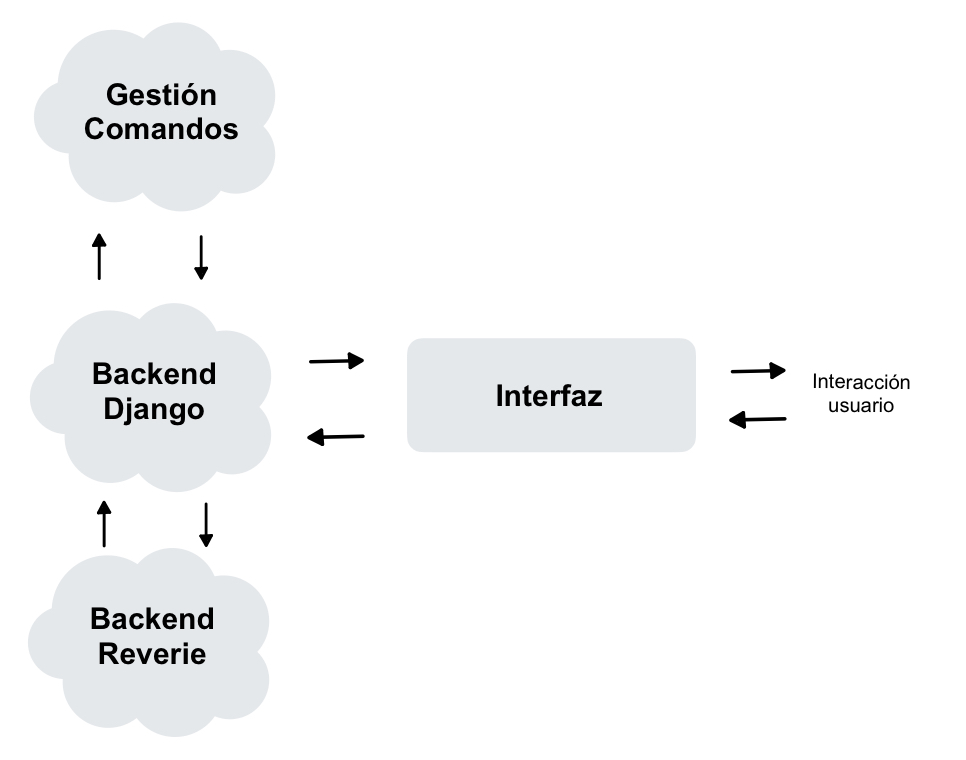
\includegraphics[width = 0.9\textwidth]{Imagenes/Vectorial/disenoSistemaFinal.jpeg}
	\caption{Diseño del sistema final tras las adaptaciones}
	\label{fig:sistemaFinal}
\end{figure}

Ahora, como se puede ver, hay un punto único de interacción entre el usuario y el sistema, que es mediante la interfaz. Así, interactuando con la interfaz los usuarios son capaces ahora de hacer lo mismo que antes y más, con las extensiones implementadas.

Mediante esta interacción, los usuarios pueden ejecutar todos los comandos, ver las simulaciones, crearlas e interactuar con ellas libremente.

El flujo de ejecución ahora es algo diferente:

\begin{enumerate}
	\item El usuario interactúa mediante la interfaz decidiendo la acción que desee
	
	\item Si el usuario desea ejecutar un comando de la simulación, se captará mediante la interfaz, se redirigirá al backend de django, el cual gestionará la llamada al gestor de comandos (nos permite ejecutar comandos mientras la aplicación sigue funcionando) y esta se encargará de llamar al backend de reverie para que ejecute el comando
	
	\item El backend de reverie devolverá la ejecución del comando a Django
	
	\item Al igual que antes, Django procesará esta información y la devolverá a la interfaz, donde el usuario podrá visualizarla y volver a interactuar con esta nueva información
	
\end{enumerate}
